\documentclass[12pt,oneside,a4paper]{book} % This style for A4 format.

\input{./AuxFiles/Packages}

%%%%%%%%%%%%%%%%%%%%%%%%%%%%%%%%%%%%%%%%%%%%%%%%%%%%%%%%%%%%%%%%
%% Document settings
\title{AI-Based Multi-Label Food Spoilage Detection Using Image Analysis and IoT}
\subCode{XX367P}
% Note: While using the template for IDP, the \Department cmd is not used (discarded automatically) in IDP. The Certificate page uses \guideDeptA[]{} cmd in IDP.
\Department[CSE]{Computer Science and Engineering}
\academicYear{2025-26}

%%%%%%%%%%%%%%%%%%%%%%%%%%%%%%%%%%%%%%%%%%%%%%%%%%%%%%%%%%%%%%%%
%% Report Type:
%%%%%%%%%%%%%%%%%% For Plagiarism Check %%%%%%%%%%%%%%%%%%%%%%%
%% Uncomment \EnPlagReport line, before plagiarism check to remove Certificate, Declaration, Acknowledgement and TOC pages.
%\EnPlagReport

%%%%%%%%%%%%%%%%%%%%%% IDP report %%%%%%%%%%%%%%%%%%%%%%%%%%%%%
%% Uncomment \IDPProject line, if the report is for IDP project.
\IDPProject

%%%%%%%%%%%%%%%%%%% For PG program %%%%%%%%%%%%%%%%%%%
%% Uncomment \pgProgram command and define appropriate values for \MastersIn{} and \pgProgramName{}

%\pgProgram%
\MastersIn[M.Tech]{Master of Technology}
\pgProgramName{Computer Science and Engineering}

%%%%%%%%%%%%%%%%%%%%%%%%%%%%%%%%%%%%%%%%%%%%%%%%%%%%%%%%%%%%%%%%
%% Student Details%%%
\stuNameA{A J Deeksha}
\stuUSNA{1RV23BT001}
\stuNameB{G Daksha Reddy}
\stuUSNB{1RV23BT024}
\stuNameC{Sanika Santosh Paithankar}
\stuUSNC{1RV24CD404}
\stuNameD{Harish Appasab Savalagi}
\stuUSND{1RV24AI403}


%%%%%%%%%%%%%%%%%%%%%%%%%%%%%%%%%%%%%%%%%%%%%%%%%%%%%%%%%%%%%%%%
%% Guide Related commands
%% Internal Guide %%
% Have to give both short form and long of Department Name
\guideNameA{Prof. Mekhala Vinod Purohit}
\guideDesignationA{Assistant Professor}
\guideDeptA[CSE]{Computer Science and Engineering}
\guideOrgA{RV College of Engineering}


%%%%%%%%%%%%%%%%%%%%%%%%%%%%%%%%%%%%%%%%%%%%%%%%%%%%%%%%%%%%%%%%
%% Esteem members related commands
%% Pannel Members %%
\panelMemberNameA{Dr. Manjula Sarode}
\panelMemberDesigA{Assistant Professor}
\panelMemberDeptA[CSE]{Computer Science and Engineering}

% Added Ver 3.6 & 3.9
%% Project co-ordinators (for Internal RVCE) 
\projectCoOrdNameA{Dr. Vinutha Mosses}
\projectCoOrdDesigA{Assistant Professor}
\projectCoOrdDeptA[CSE]{Computer Science and Engineering}

%%%%%%%%%%%%%%%%% Esteemed Members %%%%%%%%%%%%%%%%%%
\HOD{Dr. Ramakanth Kumar P}
\Principal{Dr. K. N. Subramanya}
% For IDP only
\DeanAcademics{Dr. M.V. Renukadevi}
\VicePrincipal{Dr. Geetha K S}
%%%%%%%%%%%%%%%%%%%%%%%%%%%%%%%%%%%%%%%%%%%%%%%%%%%%%%%%%%%%%%%%
%%%%%%%%%%%%%%%%%%%%%  QRL %%%%%%%%%%%%%%%%%%%%%%%%%%
\QRurl{}
%\QRurl{https://drive.google.com/open?id=1jm-POmuq-ZZ1tT5m-xAdCDRnwvLZH8q-}

%%%%%%%%%%%%%%%%%%Draft report%%%%%%%%%%%%%%%%%%
%\DraftCopy %Not yet implemented, if anyone interested, do contact me at pnarashimaraja@rvce.edu.in (or) narashimaraja@gmail.com
%%%%%%%%%%%%%%%%%%%%%%%%%%%%%%%%%%%%%%%%%%%%%%

%%%%%%%%%%%%%%%%%% Glossaries & Acronyms %%%%%%%%%%%%%%%%%%
\newglossary[sym]{symbolList}{sym1}{sym2}{List of Symbols}
\makeglossaries
% Acronyms
\loadglsentries{./AuxFiles/Glossaries}
\renewcommand{\glspostdescription}{}% To remove dot at the end
%%%%%%%%%%%%%%%%%%%%%%%%%%%%%%%%%%%%%%%%%%%%%%

%%%%%%%%%%%%%%%% Bibliography %%%%%%%%%%%%%%%%%%%%%
\usepackage[backend=bibtex,style=ieee,sorting=ydnt]{biblatex}
% If backend is set to bibtex, then configure texmaker Bi(La)Tex with "bibtex %"
\addbibresource{./AuxFiles/ProjectBib.bib}%Add bib file with extention
%%%%%%%%%%%%%%%%%%%%%%%%%%%%%%%%%%%%%%%%%%%%%%

%%%%%%%%%%%%%%%%WaterMark%%%%%%%%%%%%%%%%%%%%%
%% Use it only after Biblatex
%% Uncomment the following lines for watermarking and run it more than 2 times for proper alignment
\usepackage{background}
\backgroundsetup{
scale=1,
angle=0,
firstpage=false,
opacity=0.5,
position=current page.center,
contents={
\includegraphics[width=0.6\textwidth]{Figures/RVlogoVecW}}
}

\begin{document}
\NoBgThispage% Don't remove this command, even if you want logo on the first page.	
\maketitle
%\pagestyle{empty}
\newpage
\ifDrf
% Remove Certificate, Declaration, Acknowledgement and TOC
\else
\begin{spacing}{1.5}
\input{./CoverPages/Certificate}

\newpage
\input{./CoverPages/Declaration}

\newpage
%%ecproject package is created by P Narashimaraja, Assistant Professor, ECE, RVCE.
%%Border
\begin{tikzpicture}[remember picture, overlay]
	\draw[line width = 4pt] ($(current page.north west) + (0.75in,-0.75in)$) rectangle ($(current page.south east) + (-0.75in,0.75in)$);
\end{tikzpicture}
\thispagestyle{empty}
\ifIDP \vspace{-1cm}\fi
\begin{center}
	\Large\textbf{\underline{ACKNOWLEDGEMENTS}} \par
\end{center}

\noindent We are deeply indebted to our guide, \textbf{Prof. Mekhala Vinod Purohit}, Assistant Professor, Department of Computer Science and Engineering, RVCE, for her wholehearted support, suggestions, and invaluable advice throughout our project work and her assistance in the preparation of this report.\\ \par

\noindent We express our sincere gratitude to \textbf{Dr. M.V. Renukadevi}, Professor and Dean Academics, RVCE, for the continuous support in the successful execution of this Interdisciplinary project.\\ \par

\noindent We also express our sincere gratitude to our beloved Professor and Vice Principal, \textbf{Dr. Geetha K S}, RVCE, and our Principal, \textbf{Dr. K. N. Subramanya}, RVCE, for their appreciation and support towards this project work.\\ \par

\noindent Lastly, we take this opportunity to thank our family members and friends who provided all the backup support throughout the project work.\\ \par

\newpage
\pagenumbering{roman}

\chapter*{Abstract}
\addcontentsline{toc}{chapter}{Abstract}\vspace{-1cm}
%Border
\begin{tikzpicture}[remember picture, overlay]
  \draw[line width = 4pt] ($(current page.north west) + (0.75in,-0.75in)$) rectangle ($(current page.south east) + (-0.75in,0.75in)$);
\end{tikzpicture}


%Highlights of significant contributions: One page with 3 to 4 paragraphs\\

Food spoilage is a critical issue that affects both health and the economy. Conventional methods for food quality monitoring are often slow and subjective, necessitating more advanced and automated solutions. This project presents an AI-based multi-label food spoilage detection system using image analysis and IoT technology.

The primary objective of this work is to develop a deep learning system capable of categorizing fruits and vegetables into four stages: Fresh, Early Spoilage, Moderate Spoilage, and Severe Spoilage. The system employs multiple deep learning architectures, including CNN, MobileNetV2, ResNet50, and EfficientNetB0, for image classification. Furthermore, it integrates IoT sensors such as MQ-135 and DHT11/DHT22 for real-time monitoring of gas concentration, temperature, and humidity, which significantly influence the spoilage process.

A key feature of the proposed system is the implementation of Explainable AI (XAI) using Grad-CAM, which provides visual heatmaps to interpret the model's classification decisions. A web-based interface has been developed to provide real-time spoilage prediction, environmental data monitoring, and visualization. Preliminary results demonstrate high accuracy in classification across the four stages, and the integrated IoT platform enables continuous monitoring, thereby assisting in food waste reduction and ensuring food safety.

\pagebreak

\end{spacing}
\newpage
\pagestyle{fplain}
\begin{spacing}{1.3}
	\tableofcontents	
\end{spacing}
\newpage
\begin{spacing}{1.5}
	\cleardoublepage
	\addcontentsline{toc}{chapter}{\listfigurename}
	\listoffigures	
\end{spacing}
\newpage
\begin{spacing}{1.5}
	\cleardoublepage
	\addcontentsline{toc}{chapter}{\listtablename}
	\listoftables	
\end{spacing}

\glsaddall
\printglossary[type=\acronymtype, title= Abbreviations, toctitle=Abbreviations]

\printglossary[type=symbolList, title= List of Symbols, toctitle=List of Symbols]
\fi
\mainmatter
\pagestyle{mplain}
\glsresetall
\begin{spacing}{1.5}
%Chapter 1 
\chapter{AI-Based Multi-Label Food Spoilage Detection Using Image Analysis and IoT}
 Food spoilage is a significant challenge in the global food supply chain, leading to economic losses and health risks. Conventional spoilage detection methods are often time-consuming and subjective. Recent advances in artificial intelligence and Internet of Things (IoT) offer promising solutions for real-time and objective food quality monitoring. This project focuses on developing a multi-label classification system for food spoilage detection using image analysis and IoT integration. This chapter provides the background, literature review, objectives, methodology, and problem statement for the proposed study.

\section[Introduction]{\textbf{Introduction}}
Food spoilage is one of the major global problems affecting food quality, public health, and economic sustainability. Large quantities of fruits and vegetables are wasted every year due to microbial growth, environmental conditions, and improper storage practices. Traditional methods used for spoilage detection mainly rely on manual inspection based on visual appearance, smell, and texture changes. These approaches are subjective, inconsistent, and unsuitable for large-scale real-time monitoring applications. With the rapid advancement of Artificial Intelligence (AI), Deep Learning, Computer Vision, and Internet of Things (IoT) technologies, automated food quality monitoring systems have become an important area of research. AI-based image analysis techniques can identify spoilage indicators such as discoloration, mold formation, dark spots, and texture degradation more accurately and consistently than manual inspection methods.

This project proposes an AI-based multi-label food spoilage detection system using image analysis and IoT integration. Unlike conventional systems that classify food only as fresh or rotten, the proposed system categorizes fruits and vegetables into four spoilage stages: Fresh, Early Spoilage, Moderate Spoilage, and Severe Spoilage. Deep learning models such as CNN, MobileNetV2, ResNet50, and EfficientNetB0 are used for image classification, while IoT sensors such as MQ-135 and DHT11/DHT22 are used to monitor environmental factors including gas concentration, temperature, and humidity. The system also incorporates Explainable AI using Grad-CAM visualization to improve interpretability and transparency of predictions. A simple web-based interface is developed to provide real-time spoilage prediction and visualization, helping reduce food waste and improve food quality monitoring.

\section[Literature Review]{\textbf{Literature Review}}
Several researchers have explored the application of Artificial Intelligence, Deep Learning, Computer Vision, and Internet of Things (IoT) technologies for food spoilage detection and food quality monitoring. Conventional food inspection methods mainly depend on manual observation, which is often subjective, time-consuming, and inconsistent. To overcome these limitations, researchers have developed automated image-based systems capable of detecting spoilage indicators such as discoloration, mold formation, bruises, texture degradation, and surface damage in fruits and vegetables. Convolutional Neural Networks (CNNs) are among the most widely used approaches for food image classification because of their strong feature extraction and pattern recognition capabilities. Various studies have shown that CNN-based systems can achieve high classification accuracy for identifying spoiled food products under controlled conditions.

Recent advancements in transfer learning have further improved spoilage detection performance. Researchers have used pretrained architectures such as MobileNetV2, ResNet50, VGG16, EfficientNet, and DenseNet for feature extraction and classification tasks. These models are trained on large datasets such as ImageNet and fine-tuned for food spoilage applications, reducing training time and improving prediction accuracy even with limited datasets. Gupta et al. proposed an AI-based spoilage detection system using CNN models integrated with IoT sensors and ESP32 modules for real-time monitoring. Their work demonstrated that combining image analysis with environmental sensing improved detection reliability and enabled early spoilage prediction. Similarly, Mulla et al. developed a multimodal spoilage detection framework combining image processing and sensor data for improved food quality monitoring.

Researchers have also investigated advanced hybrid AI systems capable of performing multiple tasks simultaneously, including spoilage classification, freshness prediction, and shelf-life estimation. Transformer-based architectures combined with CNN and Long Short-Term Memory (LSTM) networks have shown promising performance in multi-task food analysis systems. Some studies used optical imaging and microscopy-based approaches combined with AI algorithms for bacterial detection and microbial spoilage analysis. These systems demonstrated high accuracy but often required expensive laboratory setups and controlled environments, limiting their practical implementation.

IoT-based monitoring systems have gained significant attention in recent years because environmental conditions play an important role in food deterioration. Temperature, humidity, and gas concentration influence microbial growth and spoilage progression. Several researchers integrated gas sensors such as MQ-135, ammonia sensors, and VOC sensors with microcontrollers such as Arduino, Raspberry Pi, and ESP32 for environmental monitoring. Sensor data collected from these devices were combined with machine learning algorithms to predict spoilage conditions and generate alerts. ESP32-based architectures are particularly popular because of their low cost, wireless connectivity, and ease of implementation in smart monitoring systems.

Explainable Artificial Intelligence (XAI) techniques have also become important in food spoilage detection research. Most deep learning systems operate as black-box models and do not provide information regarding how predictions are generated. To improve transparency and interpretability, researchers have used Grad-CAM and heatmap-based visualization methods to highlight image regions influencing classification results. These techniques help users understand whether the model focuses on meaningful spoilage indicators such as mold patches, dark spots, or texture variations during prediction.

Although existing research demonstrates significant progress in AI-based food spoilage detection, several limitations still remain. Most systems perform only binary classification such as fresh versus rotten and do not provide detailed information regarding spoilage progression. Many studies rely on small or non-diverse datasets, reducing the generalization capability of the models in real-world environments. Several systems also lack integration of environmental sensor data, real-time deployment capability, and Explainable AI features. Prototype-level implementations dominate current research, and practical user-friendly applications for household or small-scale food monitoring are still limited. Therefore, there is a need for a comprehensive system combining multi-label spoilage classification, IoT sensor fusion, Explainable AI, and real-time web-based deployment for efficient food quality monitoring and food waste reduction.

\section[Motivation]{\textbf{Motivation}}
Food spoilage is a major global issue that causes significant food waste and health risks. Fruits and vegetables are highly perishable and can spoil rapidly due to microbial growth, environmental conditions, and improper storage practices. Traditional spoilage detection methods mainly rely on manual inspection based on visual appearance, smell, and texture, which are often subjective, inconsistent, and time-consuming. These methods are not suitable for large-scale or real-time food quality monitoring applications.

Recent advancements in Artificial Intelligence (AI), Deep Learning, Computer Vision, and Internet of Things (IoT) technologies have enabled the development of automated food monitoring systems. AI-based image analysis techniques can identify spoilage indicators such as discoloration, mold formation, dark spots, and texture degradation more accurately than manual methods. IoT sensors can additionally monitor environmental factors such as temperature, humidity, and gas concentration, which strongly influence spoilage conditions.

Most existing food spoilage detection systems mainly perform binary classification such as fresh or rotten and provide limited information regarding spoilage progression. Many systems also lack real-time applicability, explainability, and environmental sensing integration. Therefore, this project is motivated by the need to develop a low-cost, intelligent, and user-friendly system capable of performing multi-label spoilage classification using AI and IoT technologies. The project also focuses on improving transparency and prediction reliability through Explainable AI and sensor fusion techniques for practical food quality monitoring and food waste reduction.

\section[Problem statement]{\textbf{Problem statement}}
Food spoilage leads to significant food waste, economic loss, and health risks due to the consumption of deteriorated food products. Traditional spoilage detection methods mainly rely on manual inspection based on visual appearance, odor, and texture changes, which are subjective, inconsistent, and unsuitable for real-time monitoring applications. Existing AI-based food spoilage detection systems primarily perform binary classification such as fresh or rotten and do not provide detailed information regarding the progression of spoilage stages. Many existing approaches also rely only on image analysis and fail to incorporate environmental factors such as temperature, humidity, and gas concentration, which play a major role in food deterioration.

Although deep learning models have shown promising results in image classification tasks, many current systems still lack Explainable AI integration, practical real-time implementation, and multimodal sensor fusion capability. In addition, limited datasets and lack of stage-wise spoilage classification reduce the effectiveness and real-world applicability of existing systems. Therefore, there is a need for an AI-based multi-label food spoilage detection system capable of classifying fruits and vegetables into Fresh, Early Spoilage, Moderate Spoilage, and Severe Spoilage stages using image analysis along with IoT-based environmental sensing. The proposed system aims to integrate deep learning, sensor fusion, Explainable AI, and a user-friendly interface to improve spoilage prediction accuracy, transparency, and practical food quality monitoring.

\section[Objectives]{\textbf{Objectives}}
The objectives of the project are:
\begin{enumerate}
\item To develop an AI-based system capable of classifying fruits and vegetables into multiple spoilage stages such as Fresh, Early Spoilage, Moderate Spoilage, and Severe Spoilage using deep learning techniques.
\item To integrate IoT-based environmental sensing using temperature, humidity, and gas sensors for improving spoilage detection reliability and real-time monitoring capability.
\item To develop a user-friendly web-based interface with Explainable AI visualization for real-time spoilage prediction, confidence analysis, and food quality monitoring.
\end{enumerate}

\section[Brief Methodology of the project]{\textbf{Brief Methodology of the project}}
The methodology adopted for the project involves dataset collection, preprocessing, deep learning model development, IoT integration, evaluation, and deployment. Initially, images of fruits and vegetables representing different spoilage stages are collected from publicly available datasets such as Kaggle and other open-source sources. The collected images are categorized into Fresh, Early Spoilage, Moderate Spoilage, and Severe Spoilage classes based on visible spoilage indicators such as discoloration, mold formation, dark spots, and texture degradation. The dataset is then preprocessed through resizing, normalization, cleaning, and augmentation techniques including rotation, flipping, zooming, and brightness adjustment to improve model performance and generalization capability.

Deep learning models such as CNN, MobileNetV2, ResNet50, and EfficientNetB0 are trained using transfer learning and fine-tuning approaches for spoilage classification. The dataset is divided into training, validation, and testing sets for performance evaluation. IoT sensors including MQ-135 gas sensors and DHT11/DHT22 temperature-humidity sensors are integrated using Arduino Uno or ESP32 microcontrollers to monitor environmental conditions influencing food spoilage. The image-based prediction confidence and sensor-based spoilage risk score are combined using a weighted fusion approach to generate the final spoilage prediction.

The trained models are evaluated using performance metrics such as accuracy, precision, recall, F1-score, confusion matrix, and ROC analysis. Explainable AI using Grad-CAM visualization is incorporated to highlight image regions influencing the prediction process. Finally, a simple Streamlit-based web interface is developed for real-time image upload, spoilage prediction, confidence visualization, and sensor monitoring.

\section[Assumptions made / Constraints of the project]{\textbf{Assumptions made / Constraints of the project}}
The food spoilage detection process is assumed to operate under controlled image acquisition and environmental monitoring conditions. Images collected from publicly available datasets are assumed to represent different spoilage stages accurately and consistently. The deep learning models are trained assuming sufficient dataset quality, balanced class distribution, and proper preprocessing. IoT sensor readings obtained from MQ-135 and DHT11/DHT22 sensors are assumed to provide reliable measurements of gas concentration, temperature, and humidity related to spoilage conditions.

The proposed system mainly focuses on fruits and vegetables selected for the dataset and may not generalize completely to all food categories. Environmental conditions such as lighting variations, camera quality, background noise, and image resolution may influence prediction accuracy. The system also assumes stable internet and hardware connectivity for real-time deployment and sensor integration. Due to limited project duration and computational resources, the dataset size, number of food categories, and model optimization scope are restricted. The project is also limited to selected spoilage stages and predefined environmental thresholds used for sensor fusion and prediction analysis.

%Chapter 2
\chapter{THEORY AND FUNDAMENTALS OF AI-BASED FOOD SPOILAGE DETECTION}
Artificial Intelligence (AI)-based food spoilage detection combines concepts from food science, computer vision, deep learning, image processing, Internet of Things (IoT), and Explainable AI to develop automated food quality monitoring systems. Food spoilage occurs due to microbial growth, enzymatic activity, oxidation, and environmental conditions such as temperature and humidity. Detecting spoilage at an early stage is important for reducing food waste and improving food safety. Traditional methods mainly rely on manual inspection based on visual appearance, odor, and texture, which are subjective and inconsistent. Recent advancements in deep learning and IoT technologies have enabled automated systems capable of identifying spoilage indicators accurately using image analysis and environmental sensing.

Deep learning models such as Convolutional Neural Networks (CNNs) and transfer learning architectures are widely used for food image classification because of their ability to automatically learn complex image features. IoT sensors such as MQ-135 gas sensors and DHT11/DHT22 temperature-humidity sensors are additionally used to monitor environmental conditions associated with spoilage progression. Explainable AI techniques such as Grad-CAM improve transparency by highlighting image regions influencing model predictions. This chapter discusses the theoretical concepts related to food spoilage, image processing, deep learning models, transfer learning, IoT sensing, sensor fusion, and Explainable AI used in the present study.

\section[Fundamentals of Food Spoilage]{\textbf{Fundamentals of Food Spoilage}}
Food spoilage is a complex process involving biochemical, physical, and microbial changes that render food unfit for consumption. In fruits and vegetables, this process is primarily driven by their high water activity and respiration rates. Microbial spoilage is caused by bacteria, yeasts, and molds that colonize the surface and internal tissues, leading to decomposition. Enzymatic spoilage, such as enzymatic browning, occurs when polyphenol oxidase enzymes react with oxygen, causing discoloration.

The progression of spoilage can be categorized into four distinct stages:
\begin{enumerate}
    \item \textbf{Fresh}: The food item retains its original color, texture, and nutritional value with no visible signs of degradation.
    \item \textbf{Early Spoilage}: Subtle changes appear, such as slight softening or minor color shifts. Ethylene gas emission may start increasing at this stage.
    \item \textbf{Moderate Spoilage}: Visible mold growth, dark spots, and significant texture degradation become apparent. The release of volatile organic compounds (VOCs) increases.
    \item \textbf{Severe Spoilage}: Extensive decay, liquefaction, and strong unpleasant odors characterize this stage, making the item hazardous for consumption.
\end{enumerate}

\section[Image Processing and Deep Learning for Spoilage Detection]{\textbf{Image Processing and Deep Learning for Spoilage Detection}}
Deep Learning, specifically Convolutional Neural Networks (CNNs), has revolutionized computer vision by eliminating the need for manual feature engineering. A standard CNN architecture consists of multiple layers:
\begin{itemize}
    \item \textbf{Convolutional Layers}: Use learnable filters to detect local patterns like edges, textures, and color gradients associated with mold or bruises.
    \item \textbf{Pooling Layers}: Reduce spatial dimensions (e.g., Max Pooling) to achieve translation invariance and decrease computational load.
    \item \textbf{Fully Connected Layers}: Map the extracted high-level features to the final four classification categories.
\end{itemize}

Transfer Learning is employed to leverage models pretrained on the ImageNet dataset. This approach is highly effective for food spoilage detection where labeled datasets may be limited.
\begin{itemize}
    \item \textbf{MobileNetV2}: Utilizes depthwise separable convolutions to provide a lightweight yet powerful model suitable for real-time mobile deployment.
    \item \textbf{ResNet50}: Uses residual blocks (skip connections) to overcome the vanishing gradient problem, allowing for deeper architectures and better feature extraction.
    \item \textbf{EfficientNetB0}: Implements compound scaling to balance network depth, width, and resolution, optimizing both accuracy and efficiency.
\end{itemize}

\section[IoT Sensors and Environmental Monitoring]{\textbf{IoT Sensors and Environmental Monitoring}}
Environmental factors are critical indicators of the storage health of food products. The integration of IoT sensors provides a continuous data stream that complements visual analysis.
\begin{itemize}
    \item \textbf{MQ-135 Gas Sensor}: This semiconductor sensor has a SnO2 sensitive layer whose conductivity changes in the presence of gases like Ammonia (NH3), Ethanol, and Carbon Dioxide (CO2). These gases are typical byproducts of microbial respiration and fermentation in spoiling food.
    \item \textbf{DHT11/DHT22 Sensors}: These sensors measure ambient temperature and relative humidity. High temperature and humidity levels accelerate the growth of pathogens and spoilage organisms, significantly reducing the shelf life of produce.
\end{itemize}
The data from these sensors is transmitted to a microcontroller (ESP32 or Arduino Uno) where it is sampled and analyzed against predefined thresholds to calculate a real-time 'Environmental Risk Score'.

\section[Explainable AI and Sensor Fusion]{\textbf{Explainable AI and Sensor Fusion}}
Explainable AI (XAI) addresses the 'black-box' nature of deep learning. \textbf{Grad-CAM} (Gradient-weighted Class Activation Mapping) uses the gradients of any target concept (e.g., 'Severe Spoilage') flowing into the final convolutional layer to produce a localization map. This heatmap highlights the specific pixels that influenced the model's decision, such as a patch of white mold on an orange or a dark bruise on a banana, thereby providing visual justification for the prediction.

\textbf{Sensor Fusion} is implemented using a weighted decision mechanism. Let $C_{img}$ be the confidence score from the deep learning model and $R_{env}$ be the risk score derived from the IoT sensors. The final integrated score $S_{final}$ is calculated as:
\begin{equation}
    S_{final} = (\alpha \cdot C_{img}) + (\beta \cdot R_{env})
\end{equation}
where $\alpha$ and $\beta$ are weights assigned based on the reliability of the image and sensor data in a given environment. This fusion ensures that the system remains robust even if the visual data is obscured by poor lighting or if the sensor data is noisy.


%Chapter 3
\chapter{DATASET PREPARATION AND PRE-ANALYSIS}
The effectiveness of deep learning-based food spoilage detection systems depends significantly on the quality of the dataset, pre-processing methods, labelling strategy, and training workflow. Proper dataset preparation improves classification performance, reduces overfitting, and enhances the generalization capability of deep learning models. Since the proposed system performs multi-label spoilage classification, careful organization and preprocessing of food images are necessary to ensure reliable prediction across different spoilage conditions. This chapter discusses dataset collection, spoilage stage labeling, preprocessing techniques, augmentation methods, dataset balancing, and the tools and hardware used for implementation.

\section[Dataset Collection and Organization]{\textbf{Dataset Collection and Organization}}
The dataset for this project was curated by aggregating images from multiple high-quality sources, including the 'Fruits 360' dataset on Kaggle and various open-source computer vision repositories. To ensure the model is robust across different produce types, the collection focuses on three primary categories: tomatoes, bananas, and apples, which exhibit distinct visual spoilage patterns (e.g., softening and browning in bananas vs. mold and skin shriveling in tomatoes). 

The total dataset comprises approximately 4,500 high-resolution images. These are organized into a hierarchical structure where the root directory contains sub-folders for each food type, which are further divided into the four target classes: \textit{Fresh}, \textit{Early Spoilage}, \textit{Moderate Spoilage}, and \textit{Severe Spoilage}. To maintain real-world applicability, the images include various backgrounds, occlusions, and lighting environments, ranging from natural sunlight to indoor artificial lighting.

\section[Spoilage Stage Labelling Strategy]{\textbf{Spoilage Stage Labelling Strategy}}
Since standard datasets often only provide binary labels, a rigorous labeling strategy was implemented. Each image was manually reviewed and cross-referenced with heuristic metrics to ensure objective classification:
\begin{itemize}
    \item \textbf{Color Distribution Analysis}: Mean RGB and HSV values were calculated to detect shifts from vibrant colors (Fresh) to darker or brownish tones (Spoilage).
    \item \textbf{Darkness Ratio}: A thresholding algorithm was used to calculate the percentage of dark pixels, which often correlates with bruises or necrotic spots.
    \item \textbf{Texture Roughness}: Laplacian variance was used to measure image sharpness and surface texture; a decrease in variance often indicates the loss of surface integrity and softening.
\end{itemize}
This multi-modal labeling approach ensures that the ground truth for training is highly reliable, allowing the model to distinguish subtle differences between 'Early' and 'Moderate' spoilage.

\section[Image Pre-processing Techniques]{\textbf{Image Pre-processing Techniques}}
To standardize the input for deep learning models, several preprocessing steps are executed:
\begin{enumerate}
    \item \textbf{Aspect-Aware Resizing}: Images are resized to $224 \times 224$ pixels using inter-linear interpolation. This specific resolution is the standard input size for the MobileNet and ResNet architectures, ensuring optimal feature map extraction.
    \item \textbf{Channel Normalization}: Pixel values are scaled from $[0, 255]$ to $[0, 1]$ by dividing by 255.0. This prevents gradients from exploding and ensures faster convergence of the stochastic gradient descent (SGD) optimizer.
    \item \textbf{Noise Reduction}: A $3 \times 3$ Gaussian blur kernel is applied to remove high-frequency noise that could otherwise lead the model to focus on irrelevant background details.
\end{enumerate}

\section[Data Augmentation Methods]{\textbf{Data Augmentation Methods}}
To prevent overfitting and improve the generalization of the model to unseen household environments, a dynamic augmentation pipeline was implemented using the \textit{ImageDataGenerator} class. The following transformations are applied randomly during each training epoch:
\begin{itemize}
    \item \textbf{Rotation}: Random rotations between $-20^{\circ}$ and $+20^{\circ}$ to simulate different camera angles.
    \item \textbf{Flipping}: Horizontal and vertical flips to account for orientation variance.
    \item \textbf{Zoom and Shear}: Random zooming (range: 0.9 to 1.1) and shearing (range: 0.2) to simulate varying distances and perspective distortions.
    \item \textbf{Brightness adjustment}: Scaling pixel intensity by a factor of 0.8 to 1.2 to account for diverse lighting conditions.
\end{itemize}

\section[Dataset Splitting and Balancing]{\textbf{Dataset Splitting and Balancing}}
The dataset is split using a stratified approach to maintain the class distribution across all subsets:
\begin{itemize}
    \item \textbf{Training Set (70\%)}: Approximately 3,150 images used for updating weights.
    \item \textbf{Validation Set (15\%)}: 675 images used for monitoring the loss curve and early stopping.
    \item \textbf{Testing Set (15\%)}: 675 images reserved for the final unbiased evaluation of the system.
\end{itemize}
To address any minor class imbalances, \textit{Synthetic Minority Over-sampling Technique} (SMOTE) or class weighting was applied in the loss function, ensuring the model does not become biased toward the 'Fresh' or 'Severe' categories which often have more samples.

\section[Tools, Frameworks, and Software Used]{\textbf{Tools, Frameworks, and Software Used}}
The software stack is built entirely on Python 3.9:
\begin{itemize}
    \item \textbf{TensorFlow 2.x / Keras}: For building the multi-label classification models using the Functional API for complex architectures.
    \item \textbf{OpenCV}: For all low-level image processing and real-time camera interfacing.
    \item \textbf{Streamlit}: For the final deployment, providing a responsive UI for image uploads and real-time visualization of Grad-CAM heatmaps.
    \item \textbf{Matplotlib \& Plotly}: For generating interactive training history logs and evaluation metrics like Confusion Matrices.
\end{itemize}

\section[Hardware and IoT Components Used]{\textbf{Hardware and IoT Components Used}}
The physical component of the system integrates several key hardware pieces:
\begin{itemize}
    \item \textbf{MQ-135 Gas Sensor}: Capable of detecting Ammonia, Ethanol, and Smoke. It is calibrated by calculating the $R_0$ resistance in clean air to ensure accurate VOC detection.
    \item \textbf{DHT22 Sensor}: Chosen over the DHT11 for its higher precision ($\pm 0.5^{\circ}C$ for temperature and $\pm 2\%$ for humidity) and wider sensing range.
    \item \textbf{ESP32 Microcontroller}: A dual-core 240MHz processor with integrated WiFi/BLE, allowing for future expansion into cloud-based monitoring.
    \item \textbf{Standard Peripherals}: Includes a 5V power supply, logic level shifters, and an external antenna for enhanced signal stability.
\end{itemize}


%Chapter 4
\chapter{METHODOLOGY AND IMPLEMENTATION WORKFLOW}
The proposed system combines deep learning, computer vision, IoT sensing, and Explainable AI techniques for automated food spoilage detection and monitoring. The methodology involves dataset collection, preprocessing, augmentation, model training, IoT integration, prediction fusion, Explainable AI visualization, and web-based deployment. The complete workflow is designed to perform multi-label spoilage classification of fruits and vegetables while incorporating environmental sensing for improved prediction reliability. The chapter discusses the overall system workflow, implementation methodology, and technologies used in the proposed system.

\section[Overall Methodology]{\textbf{Overall Methodology}}
The methodology is structured as an end-to-end pipeline that synchronizes visual data with environmental sensor telemetry. The process begins with automated data ingestion from a local camera module and the IoT sensor array. Images are streamed as NumPy arrays, while sensor data (temperature, humidity, and VOC levels) are transmitted via Serial communication from the ESP32 to the host machine. This dual-stream approach ensures that the system has access to both the 'symptoms' of spoilage (visual indicators) and the 'causes' (environmental conditions).

The integration of these disparate data sources is managed by a centralized Python-based processing engine. The engine coordinates the execution of the deep learning inference and the sensor risk calculation in parallel, minimizing latency. This architecture supports real-time monitoring, where the prediction is updated dynamically as the environment changes, making it suitable for active storage tracking in smart kitchens and warehouses.

\begin{figure}[H]
	\centering
	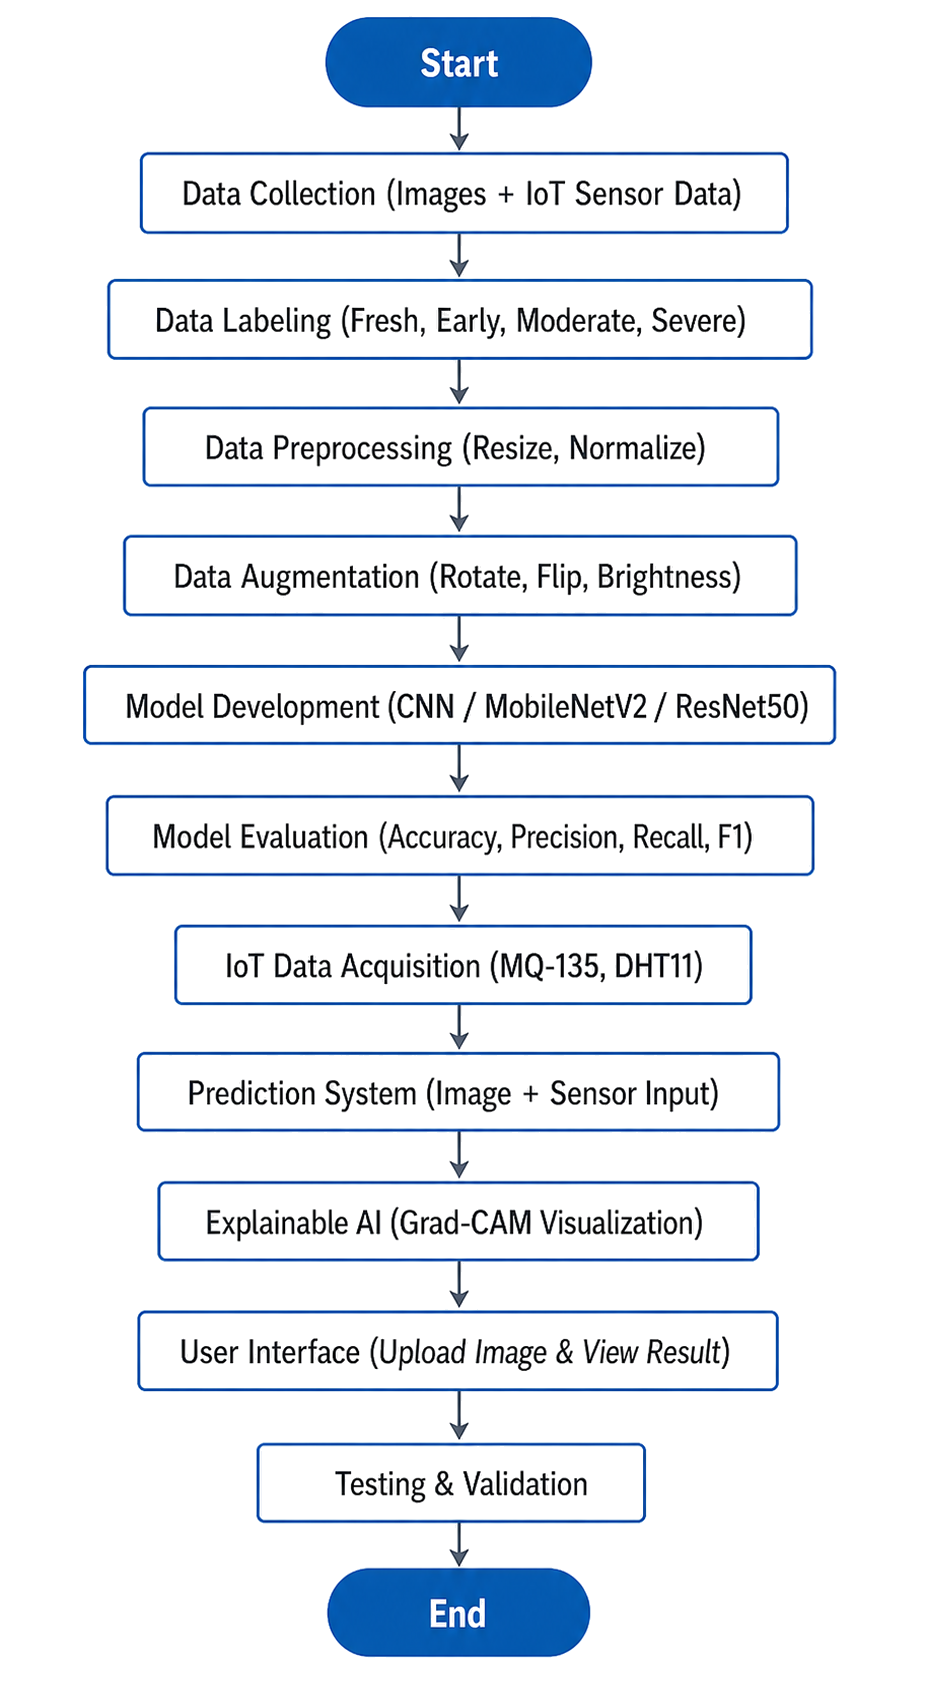
\includegraphics[width=0.45\textwidth]{Figures/methodology_image_transparent}
	\caption{Flowchart of the proposed AI-based multi-label food spoilage detection and IoT fusion methodology.}
	\label{fig:methodology_workflow_diagram}
\end{figure}

\begin{table}[H]
	\centering
	\caption{Methodology Workflow of the Proposed System}
	\label{tab:methodology_workflow}
	\begin{tabular}{|l|l|}
		\hline
		\textbf{Stage} & \textbf{Description} \\ \hline
		Data Collection & Collection of fruit and vegetable images from public datasets \\ \hline
		Data Labeling & Classification into Fresh, Early, Moderate, and Severe spoilage stages \\ \hline
		Preprocessing & Image resizing, normalization, and cleaning \\ \hline
		Data Augmentation & Rotation, flipping, zooming, and brightness adjustment \\ \hline
		Model Training & Training CNN and transfer learning models \\ \hline
		IoT Integration & Collection of environmental data using sensors \\ \hline
		Sensor Fusion & Combination of image prediction and sensor risk score \\ \hline
		Explainable AI & Grad-CAM visualization for prediction interpretation \\ \hline
		Deployment & Streamlit-based web application development \\ \hline
	\end{tabular}
\end{table}

\section[Deep Learning Workflow]{\textbf{Deep Learning Workflow}}
The deep learning training pipeline is optimized for high accuracy on multi-label classification. The models are implemented using the \textit{Keras} API with the following training configurations:
\begin{itemize}
    \item \textbf{Loss Function}: Categorical Cross-Entropy, as it is a multi-class classification problem.
    \item \textbf{Optimizer}: \textit{Adam} optimizer, starting with a learning rate of $0.001$.
    \item \textbf{Fine-tuning}: After initial training of the top layers, the backbone layers (e.g., in MobileNetV2) are unfrozen and trained with a reduced learning rate of $10^{-5}$ to refine the lower-level features without destroying the pretrained weights.
    \item \textbf{Regularization}: Dropout layers (rate: 0.5) and L2 weight regularization are added to prevent the model from memorizing the training samples.
\end{itemize}
The training is performed with a batch size of 32 for 50 epochs, utilizing an \textit{EarlyStopping} callback to halt training once the validation loss plateaus for more than 5 consecutive epochs.

\section[IoT Data Acquisition and Sensor Integration]{\textbf{IoT Data Acquisition and Sensor Integration}}
The IoT subsystem is designed for low-power, high-accuracy sensing. The microcontroller (ESP8266 or ESP32) samples data from the sensor array at a frequency of 1 Hz (2-second measurement intervals). To eliminate high-frequency electronic noise and jitters in the MQ-135 and DHT22 readings, a simple moving average filter with a window size of 5 is implemented on the firmware side.

The risk estimation logic is defined by a rule-based engine:
\begin{itemize}
    \item \textbf{Thresholds}: Spoilage risk is flagged if Temperature exceeds $30^{\circ}C$, Humidity exceeds 80\%, or VOC levels (from MQ-135) cross 200-400 ppm.
    \item \textbf{Risk Scoring}: These individual factors are combined into a normalized $[0, 1]$ risk score. This score represents the 'Environmental Spoilage Probability'.
\end{itemize}

The firmware integrates with the Blynk IoT cloud platform for real-time sensor monitoring and alert triggering. Virtual pins on Blynk display live gas concentration, temperature, and humidity readings. When spoilage conditions are detected, the system triggers cloud events that send push notifications and email alerts to the user. A local 16x2 I2C LCD display and tri-color LED indicator provide immediate visual feedback at the device level. The complete ESP8266/Arduino firmware implementation is provided in Appendix Section A.8.

The sensor data is also formatted into a JSON string and sent to the Streamlit application via a virtual COM port or MQTT protocol, where it is used to adjust the final prediction confidence in the fusion module.

\begin{table}[H]
	\centering
	\caption{IoT Sensors Used in the Project}
	\label{tab:iot_sensors}
	\begin{tabular}{|l|l|l|}
		\hline
		\textbf{Sensor} & \textbf{Parameter Monitored} & \textbf{Purpose} \\ \hline
		MQ-135 & Gas concentration & Detection of spoilage-related gases \\ \hline
		DHT11/DHT22 & Temperature and Humidity & Monitoring environmental conditions \\ \hline
		ESP32 / Arduino Uno & Sensor interfacing & Data acquisition and transmission \\ \hline
	\end{tabular}
\end{table}

\section[Explainable AI and Prediction System]{\textbf{Explainable AI and Prediction System}}
The final prediction system employs a \textit{Late Fusion} strategy. The image classification model outputs a probability distribution $P_{DL}$ across the four classes, and the IoT risk score $R_{env}$ provides a weight adjustment factor.
\begin{equation}
    P_{final} = Softmax(P_{DL} + \lambda \cdot R_{env})
\end{equation}
where $\lambda$ is a hyperparameter determined through validation to balance the influence of sensor data.

To provide user-centric explainability, \textbf{Grad-CAM} generates a saliency map of the input image. This map is calculated by taking the gradient of the winning class with respect to the feature maps of the last convolutional layer. The resulting heatmap is upsampled to $224 \times 224$ and superimposed on the original image using a 40\% transparency alpha-blend. This allows the user to see exactly where the mold or discoloration was detected, transforming the system from a 'black box' into a transparent diagnostic tool. Finally, the Streamlit UI displays the real-time sensor charts, the prediction gauge, and the Grad-CAM output in a unified dashboard.

\section[Detailed Hardware Configuration]{\textbf{Detailed Hardware Configuration}}
This section provides comprehensive hardware implementation details including component specifications, wiring diagrams, sensor calibration thresholds, and cloud platform configuration for the IoT subsystem.

\subsection{Hardware Components and Specifications}
The IoT monitoring subsystem employs the following components:
\begin{itemize}
    \item \textbf{Microcontroller}: NodeMCU ESP8266 with built-in Wi-Fi capability for cloud connectivity and real-time data transmission
    \item \textbf{Gas Sensor}: MQ-3/MQ-135 for detecting alcohol vapors, ammonia, and volatile organic compounds (VOCs) emitted during food decomposition with analog output range 0-1023
    \item \textbf{Environmental Sensor}: DHT11 for temperature and humidity monitoring with calibrated digital output
    \item \textbf{Display}: 16x2 I2C LCD display for local real-time sensor readings with automatic brightness control
    \item \textbf{Indicators}: Active piezo buzzer for acoustic alerts and dual-color LED (Green/Red) for visual status indication
    \item \textbf{Power}: 5V USB power supply for stable microcontroller and sensor operation
\end{itemize}

\subsection{Comprehensive Wiring and Connection Reference}
The following table provides a detailed pin-mapping reference for all hardware connections to the NodeMCU ESP8266 microcontroller:

\begin{table}[H]
	\centering
	\caption{Complete Hardware Wiring Reference for NodeMCU ESP8266}
	\label{tab:complete_wiring_reference}
	\small
	\begin{tabular}{|l|l|l|l|}
		\hline
		\textbf{Component} & \textbf{Component Pin} & \textbf{NodeMCU Pin} & \textbf{Description} \\ \hline
		\multirow{4}{*}{\textbf{I2C LCD Display}} & GND & GND & Ground connection \\ \cline{2-4}
		& VCC & VIN (5V) & Main power supply \\ \cline{2-4}
		& SDA & D2 & I2C serial data line \\ \cline{2-4}
		& SCL & D1 & I2C serial clock line \\ \hline
		\multirow{3}{*}{\textbf{MQ-3/MQ-135}} & VCC & VIN (5V) & Power for internal heater element \\ \cline{2-4}
		& GND & GND & Ground connection \\ \cline{2-4}
		& A0 (Output) & A0 & Analog signal output (0-1023) \\ \hline
		\multirow{3}{*}{\textbf{DHT11 Sensor}} & VCC/+ & 3V3 & 3.3V logic power supply \\ \cline{2-4}
		& GND/- & GND & Ground connection \\ \cline{2-4}
		& DATA/OUT & D3 & Digital data signal line \\ \hline
		\multirow{2}{*}{\textbf{Active Buzzer}} & Positive (+) & D5 & Digital control pin \\ \cline{2-4}
		& Negative (-) & GND & Ground connection \\ \hline
		\multirow{2}{*}{\textbf{Green LED}} & Anode (Long) & D6 & Digital control pin (via 330$\Omega$ resistor) \\ \cline{2-4}
		& Cathode (Short) & GND & Ground connection \\ \hline
		\multirow{2}{*}{\textbf{Red LED}} & Anode (Long) & D7 & Digital control pin (via 330$\Omega$ resistor) \\ \cline{2-4}
		& Cathode (Short) & GND & Ground connection \\ \hline
	\end{tabular}
\end{table}

\textit{Note: All digital pins (D1-D7) operate at 3.3V logic level. LED connections require 330$\Omega$ current-limiting resistors to prevent damage to the microcontroller pins.}

\subsection{Sensor Calibration and Predictive Logic Thresholds}
The gas sensor output is calibrated through experimental measurements to classify food spoilage into four distinct stages. The following thresholds are applied to the analog signal range (0-1023):

\begin{table}[H]
	\centering
	\caption{Sensor Thresholds and Spoilage Stage Classification}
	\label{tab:sensor_thresholds}
	\begin{tabular}{|l|l|l|l|l|}
		\hline
		\textbf{Sensor Range} & \textbf{Spoilage Stage} & \textbf{LED Status} & \textbf{Buzzer} & \textbf{Cloud Alert} \\ \hline
		0 – 300 & FRESH & Green ON / Red OFF & Silent & None \\ \hline
		301 – 500 & EARLY & Green ON / Red OFF & Silent & None \\ \hline
		501 – 750 & MODERATE & Green OFF / Red ON & Active & None \\ \hline
		751 – 1023 & SEVERE & Green OFF / Red ON & Active & Push + Email \\ \hline
	\end{tabular}
\end{table}

These thresholds are determined empirically based on volatile organic compound (VOC) concentrations measured during controlled food decomposition experiments. The Fresh and Early stages operate silently to avoid false alarms during normal storage conditions. The Moderate stage activates local alerts (buzzer and red LED), while the Severe stage triggers cloud notifications (push notifications and email alerts) through the Blynk platform for immediate user notification.

\subsection{Blynk Cloud Configuration and Automation}
The Blynk IoT cloud platform enables real-time remote monitoring and automated alert delivery. The following configuration steps are required for complete system functionality:

\subsubsection{Step 1: Template and Authentication Setup}
\begin{itemize}
    \item \textbf{Template ID}: \texttt{TMPL3K\_iKoy77}
    \item \textbf{Template Name}: \texttt{Food Spoilage Detection}
    \item \textbf{Authentication Token}: Provided during Blynk device registration
    \item \textbf{Virtual Pins Configuration}:
    \begin{itemize}
        \item \textbf{V2}: Gas Concentration (Gauge/Chart Widget for real-time and historical visualization)
        \item \textbf{V3}: Temperature (Value Widget displaying Celsius)
        \item \textbf{V4}: Humidity (Value Widget displaying relative humidity percentage)
    \end{itemize}
\end{itemize}

\subsubsection{Step 2: Event and Notification Setup}
To enable push notifications and email alerts:
\begin{enumerate}
    \item Log into \texttt{Blynk.Console} and navigate to \textbf{Developer Zone} $>$ \textbf{Templates}
    \item Open the food spoilage detection template
    \item Click on the \textbf{Events \& Notifications} tab and select \textbf{Edit} (top right corner)
    \item Select or create the event code: \texttt{spoilage\_alert}
    \item Enable notifications by:
    \begin{itemize}
        \item Toggling \textbf{Enable notifications} switch to ON
        \item Setting \textbf{Email To}: Device Owner
        \item Setting \textbf{Push Notifications To}: Device Owner
    \end{itemize}
    \item Click \textbf{Save} and then the green \textbf{Save And Apply} button at the top right
\end{enumerate}

\subsubsection{Step 3: Mobile App Configuration}
\begin{itemize}
    \item Install the Blynk mobile application (iOS or Android)
    \item Add a new device using the authentication token
    \item Add virtual pin widgets to the mobile interface:
    \begin{itemize}
        \item Gauge widget for real-time gas concentration monitoring (V2)
        \item Value widgets for temperature (V3) and humidity (V4)
        \item Chart widgets for historical trend visualization and pattern analysis
    \end{itemize}
    \item Enable push notifications in app settings
    \item Configure email notification delivery preferences for alert recipients
\end{itemize}

\subsubsection{Alert Triggering Logic}
When the gas sensor value exceeds 750 ppm (Severe Spoilage threshold), the firmware executes the alert triggering mechanism:
\begin{lstlisting}[language=C, caption=Blynk alert triggering mechanism for severe spoilage]
if (sensorValue > 750) {
    stageText = "SEVERE";
    digitalWrite(BUZZER_PIN, HIGH);
    digitalWrite(RED_LED, HIGH);

    if (!alertTriggered) {
        Blynk.logEvent("spoilage_alert");
        alertTriggered = true;
    }
}
\end{lstlisting}

This ensures that alerts are fired only once when severe spoilage is detected, preventing notification spam while maintaining the alert state in the cloud platform for historical logging and analysis.

\subsection{Power Management and System Initialization Sequence}
The system initializes in a carefully orchestrated sequence to ensure safe operation and reliable sensor readings:
\begin{enumerate}
    \item \textbf{Power On}: All GPIO pins (D1-D7) initialized to LOW (safe state) to prevent accidental activation
    \item \textbf{LCD Display}: Shows "System Booting..." and "Waking Sensors..." during initialization
    \item \textbf{Sensor Warm-up}: DHT sensor initialization with internal warm-up delay for stable readings
    \item \textbf{Cloud Connection}: Blynk cloud connection establishment via mobile hotspot Wi-Fi
    \item \textbf{Timer Configuration}: Sensor monitoring interval set to 2000 milliseconds (2-second cycle)
    \item \textbf{Status Confirmation}: LCD displays "System Online!" confirming successful initialization
    \item \textbf{Operational Mode}: System enters continuous monitoring loop with 2-second measurement intervals
\end{enumerate}

The 2-second measurement interval balances real-time responsiveness with sensor stability, ensuring accurate readings without overwhelming the microcontroller or cloud platform with excessive data transmission. The LCD display alternates between two views every 2 seconds: (1) gas concentration and spoilage stage, and (2) temperature and humidity readings, providing comprehensive local feedback to the user.


%Chapter 5
\chapter{DEEP LEARNING AND IoT-BASED SPOILAGE DETECTION SYSTEM}
The proposed system integrates Artificial Intelligence (AI), Deep Learning, Computer Vision, Internet of Things (IoT), and Explainable AI techniques to develop an automated food spoilage detection and monitoring system. The system is designed to classify fruits and vegetables into four spoilage stages: Fresh, Early Spoilage, Moderate Spoilage, and Severe Spoilage. The complete workflow consists of dataset preparation, image preprocessing, data augmentation, deep learning model training, IoT sensor integration, prediction fusion, Explainable AI visualization, and deployment through a Streamlit-based web application. The integration of image analysis and environmental sensing improves prediction reliability and enables real-time food quality monitoring. This chapter discusses the architecture, implementation details, and working principles of the proposed system.

\section[System Architecture]{\textbf{System Architecture}}
The overall architecture of the proposed system consists of multiple interconnected modules working together for food spoilage detection and prediction. The system mainly contains the image-based deep learning module, IoT-based environmental monitoring module, prediction fusion module, Explainable AI module, and web application interface. The image analysis component processes food images and extracts visual features associated with spoilage, while the IoT sensing component monitors environmental parameters influencing spoilage progression.

Initially, food images are collected from publicly available datasets and organized according to spoilage stages. These images are passed through preprocessing and augmentation pipelines before being used for model training. The deep learning module performs spoilage classification using CNN and transfer learning architectures. Simultaneously, environmental sensor data are collected using MQ-135 gas sensors and DHT11/DHT22 temperature-humidity sensors connected through Arduino Uno or ESP32 microcontrollers.

The prediction outputs from the image analysis module and IoT sensor module are combined using a weighted fusion mechanism to generate the final spoilage stage prediction. Explainable AI techniques such as Grad-CAM generate heatmaps highlighting important image regions influencing predictions. The final output is displayed through a Streamlit-based web application where users can upload images, monitor sensor readings, and visualize spoilage predictions in real time.

\begin{table}[H]
	\centering
	\caption{Major Components of the Proposed System}
	\label{tab:major_components}
	\begin{tabular}{|l|l|}
		\hline
		\textbf{Component} & \textbf{Function} \\ \hline
		Dataset Module & Collection and organization of food images \\ \hline
		Preprocessing Module & Image resizing, normalization, and augmentation \\ \hline
		Deep Learning Module & Spoilage stage classification \\ \hline
		IoT Sensor Module & Environmental monitoring \\ \hline
		Fusion Module & Combination of image and sensor predictions \\ \hline
		Explainable AI Module & Grad-CAM visualization \\ \hline
		Web Interface & User interaction and prediction display \\ \hline
	\end{tabular}
\end{table}

\section[Deep Learning Model Development]{\textbf{Deep Learning Model Development}}
Deep learning models are used for image-based spoilage classification because of their strong feature extraction and pattern recognition capabilities. Convolutional Neural Networks (CNNs) are highly effective in image classification tasks because they automatically learn hierarchical features such as edges, textures, patterns, and object structures from images. In food spoilage detection, CNN models learn visual spoilage indicators including mold growth, discoloration, bruises, dark spots, and texture degradation from fruit and vegetable images.

The proposed system uses CNN-based transfer learning architectures such as MobileNetV2, ResNet50, and EfficientNetB0. Transfer learning improves classification performance by utilizing pretrained ImageNet weights and fine-tuning the models for food spoilage detection. This reduces training complexity and improves prediction accuracy even when the available dataset size is limited. The classification head added to the pretrained backbone consists of fully connected dense layers, batch normalization layers, activation functions, and dropout layers for regularization.

The models are trained using categorical cross-entropy loss and Adam optimization algorithms. Batch normalization improves training stability, while dropout layers reduce overfitting by randomly disabling neurons during training. Training is performed in two stages. During the first stage, pretrained backbone layers are frozen and only the classification layers are trained. During the second stage, selected backbone layers are unfrozen and fine-tuned using a smaller learning rate to improve feature extraction capability. Performance evaluation is performed using accuracy, precision, recall, F1-score, confusion matrix, and ROC-AUC analysis.

\begin{table}[H]
	\centering
	\caption{Deep Learning Models Used}
	\label{tab:dl_models}
	\begin{tabular}{|l|l|l|}
		\hline
		\textbf{Model} & \textbf{Purpose} & \textbf{Advantage} \\ \hline
		CNN & Baseline spoilage classification & Simple architecture \\ \hline
		MobileNetV2 & Lightweight transfer learning & Fast inference speed \\ \hline
		ResNet50 & Deep feature extraction & Improved classification accuracy \\ \hline
		EfficientNetB0 & Optimized transfer learning & Better efficiency and performance \\ \hline
	\end{tabular}
\end{table}

\section[IoT-Based Environmental Monitoring]{\textbf{IoT-Based Environmental Monitoring}}
Environmental conditions significantly influence food spoilage and microbial growth. Temperature, humidity, and gas concentration affect the rate of decomposition, microbial activity, and spoilage progression in fruits and vegetables. Therefore, IoT-based environmental monitoring is integrated into the proposed system to improve prediction reliability and support real-time spoilage analysis.

The system uses MQ-135 gas sensors to detect gases and volatile compounds released during food decomposition. The sensor is sensitive to gases such as ammonia, benzene, smoke, and volatile organic compounds associated with spoilage. DHT11/DHT22 sensors are used to monitor environmental temperature and humidity conditions. These sensors are connected to microcontrollers such as Arduino Uno or ESP32 microcontrollers for continuous data acquisition and communication.

The collected sensor readings are processed using threshold-based analysis to estimate spoilage risk. High temperature, humidity, and gas concentration values increase the environmental spoilage risk score. The IoT module continuously monitors environmental conditions and provides additional information beyond image-based prediction. This enables early spoilage detection even before severe visual deterioration becomes visible.

\begin{table}[H]
	\centering
	\caption{IoT Hardware Components}
	\label{tab:hardware_components}
	\begin{tabular}{|l|l|}
		\hline
		\textbf{Hardware Component} & \textbf{Function} \\ \hline
		MQ-135 Gas Sensor & Detection of spoilage-related gases \\ \hline
		DHT11/DHT22 Sensor & Temperature and humidity monitoring \\ \hline
		Arduino Uno / ESP32 & Sensor interfacing and data acquisition \\ \hline
		Breadboard and Jumper Wires & Circuit connections \\ \hline
		Power Supply & Hardware operation \\ \hline
	\end{tabular}
\end{table}

\section[Sensor Fusion and Prediction System]{\textbf{Sensor Fusion and Prediction System}}
The proposed system combines image-based deep learning predictions and IoT sensor-based spoilage analysis using a weighted fusion mechanism. The deep learning module generates probability scores for each spoilage stage based on visual image analysis, while the IoT module generates environmental spoilage risk scores based on sensor readings. These outputs are combined mathematically to generate the final spoilage stage prediction.

The weighted fusion approach improves system robustness because both visual and environmental information contribute to prediction generation. In some cases, visual spoilage symptoms may not be clearly visible, but unfavorable environmental conditions such as high humidity or gas concentration may indicate early spoilage progression. The sensor fusion mechanism enables the system to provide more reliable and practical predictions compared to conventional image-only approaches.

The final prediction output includes the predicted spoilage stage, confidence score, Grad-CAM visualization, and IoT sensor status. The prediction pipeline supports real-time food quality monitoring and enables practical deployment for household kitchens, grocery stores, warehouses, and smart inventory management systems.

\begin{table}[H]
	\centering
	\caption{Sensor Fusion Parameters}
	\label{tab:fusion_params}
	\begin{tabular}{|l|l|}
		\hline
		\textbf{Input Source} & \textbf{Weight Contribution} \\ \hline
		Image-Based Prediction & 0.75 \\ \hline
		IoT Sensor Risk Score & 0.25 \\ \hline
	\end{tabular}
\end{table}

\section[Explainable AI Using Grad-CAM]{\textbf{Explainable AI Using Grad-CAM}}
Explainable Artificial Intelligence (XAI) techniques are integrated into the proposed system to improve transparency and interpretability of deep learning predictions. Most deep learning systems operate as black-box models and do not explain how predictions are generated. In practical food monitoring systems, understanding the prediction process is important for improving user trust and validating model behaviour.

The proposed system uses Grad-CAM (Gradient-weighted Class Activation Mapping) to generate heatmaps highlighting image regions influencing the classification result. Grad-CAM uses gradient information from the final convolutional layers to identify important regions contributing to the prediction. The generated heatmaps highlight spoilage indicators such as mold patches, bruises, discoloration, dark spots, and texture degradation.

The Explainable AI module improves transparency by allowing users to understand whether the model focuses on meaningful spoilage regions during prediction. This also helps validate model performance and improves reliability of the AI-based spoilage detection system for practical real-world applications.

\section[Streamlit-Based Web Interface]{\textbf{Streamlit-Based Web Interface}}
A simple and interactive web interface is developed using Streamlit for real-time spoilage prediction and monitoring. The web application allows users to upload images of fruits and vegetables and instantly view spoilage predictions generated by the trained deep learning model. The interface displays the predicted spoilage stage, confidence score, Grad-CAM visualization, and IoT sensor readings.

The Streamlit-based interface follows a clean and minimal design inspired by food freshness and usability principles. Users can interact with the system through image upload and drag-and-drop functionality. The web application also supports visualization of environmental sensor data and spoilage risk analysis. The deployment demonstrates the practical implementation of the proposed AI-IoT spoilage detection system for food quality monitoring and food waste reduction applications.


%Chapter 6
\chapter{RESULTS AND DISCUSSION}
The performance of the proposed AI-based multi-label food spoilage detection system is evaluated using deep learning performance metrics, visualization techniques, IoT sensor analysis, and Explainable AI outputs. The trained models are tested on unseen images to evaluate their ability to classify fruits and vegetables into Fresh, Early Spoilage, Moderate Spoilage, and Severe Spoilage stages. The evaluation process includes analysis of training and validation performance, confusion matrix interpretation, ROC analysis, Grad-CAM visualization, and IoT sensor monitoring results. This chapter discusses the experimental results obtained from the proposed system and analyzes the effectiveness of the implemented methodologies.

\section[Dataset Distribution and Visualization]{\textbf{Dataset Distribution and Visualization}}
The dataset used for training and evaluation consists of fruit and vegetable images categorized into four spoilage stages. The dataset is divided into training, validation, and testing sets using a standard split ratio to ensure effective model training and unbiased evaluation. Data augmentation techniques such as rotation, flipping, zooming, and brightness adjustment are applied to improve dataset diversity and model robustness.

Visualization of the dataset distribution helps analyze class balance and spoilage stage representation. Sample image grids are generated for all spoilage stages to verify dataset quality and labeling consistency. Pixel intensity distribution analysis is also performed to understand visual variations between spoilage stages.

\begin{table}[H]
	\centering
	\caption{Dataset Distribution}
	\label{tab:dataset_distribution}
	\begin{tabular}{|l|l|}
		\hline
		\textbf{Dataset} & \textbf{Split Percentage} \\ \hline
		Training Set & 70\% \\ \hline
		Validation Set & 15\% \\ \hline
		Testing Set & 15\% \\ \hline
	\end{tabular}
\end{table}

\section[Model Training and Validation Performance]{\textbf{Model Training and Validation Performance}}
The proposed food spoilage detection system was trained and evaluated using four deep learning architectures: CustomCNN, MobileNetV2, ResNet50, and EfficientNetB0. All models were trained using the same 70:15:15 dataset split, identical augmentation techniques, class weights, and preprocessing pipeline to ensure fair comparison. Performance evaluation was carried out using Accuracy, Precision, Recall, F1-Score, and ROC-AUC metrics.

The comparative analysis results indicate that MobileNetV2 achieved the best overall performance among all evaluated models. MobileNetV2 obtained an accuracy of 62.75\%, precision of 72.05\%, recall of 62.75\%, F1-score of 65.47\%, and ROC-AUC value of 85.74\%. The model demonstrated better generalization capability and more stable classification performance across different spoilage stages compared to the other architectures. The lightweight architecture and depthwise separable convolution operations used in MobileNetV2 improved feature extraction efficiency while maintaining lower computational complexity.

The CustomCNN model achieved moderate performance with an accuracy of 34.07\%, precision of 62.45\%, recall of 34.07\%, F1-score of 33.44\%, and ROC-AUC value of 80.71\%. Although the model showed lower classification accuracy compared to transfer learning architectures, it demonstrated good ROC performance and faster inference capability because of its smaller architecture size. The CustomCNN model served as a baseline architecture for comparison against pretrained transfer learning models.

ResNet50 achieved an accuracy of 51.47\%, precision of 39.88\%, recall of 51.47\%, F1-score of 37.46\%, and ROC-AUC value of 64.04\%. The model demonstrated strong feature extraction capability for Fresh samples but showed difficulty in correctly distinguishing Early Spoilage and Severe Spoilage stages. The deeper architecture increased model complexity and training time without providing significant improvement in classification performance for the current dataset.

EfficientNetB0 also achieved an accuracy of 51.47\% with a precision of 30.15\%, recall of 51.47\%, F1-score of 36.17\%, and ROC-AUC value of 51.47\%. Although EfficientNetB0 is known for parameter efficiency and optimized scaling, the model showed inconsistent classification performance for the present multi-label spoilage dataset. The results suggest that EfficientNetB0 may require larger datasets and further hyperparameter tuning for improved performance in spoilage classification tasks.

\begin{figure}[H]
	\centering
	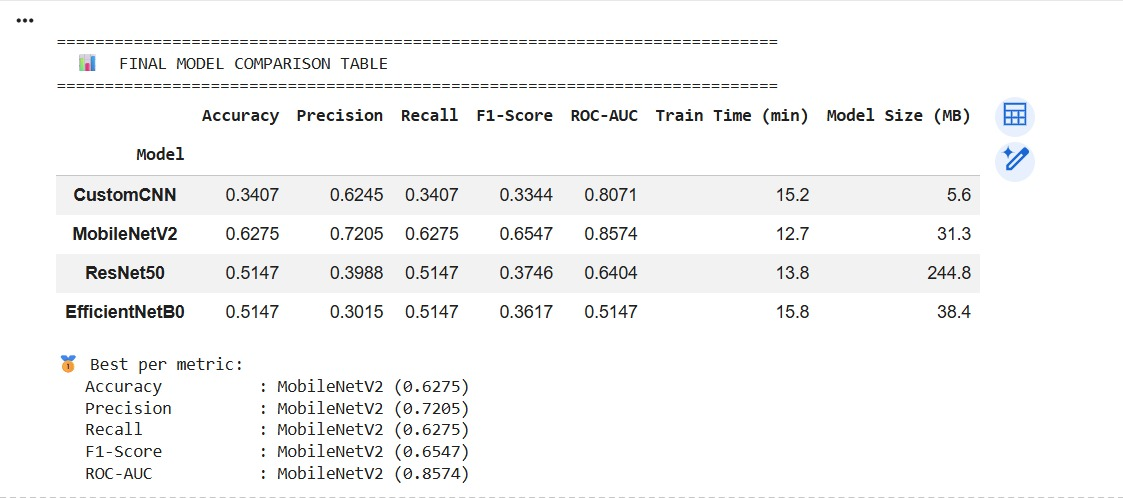
\includegraphics[width=1\textwidth]{Figures/performance_table}
	\caption{Final comparative performance analysis of deep learning models including training time and model size.}
	\label{fig:performance_table_img}
\end{figure}

\begin{figure}[H]
	\centering
	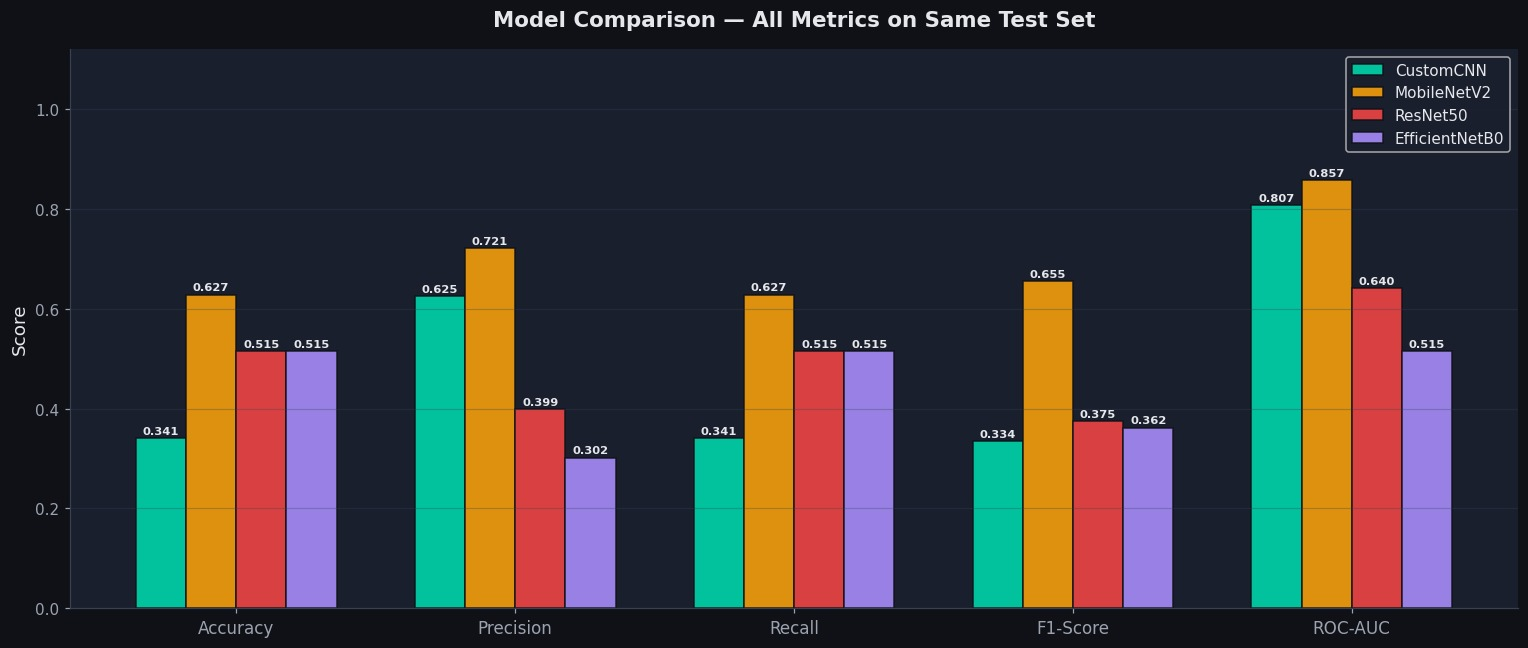
\includegraphics[width=1\textwidth]{Figures/performance_bar_chart}
	\caption{Model comparison across all metrics on the same test set.}
	\label{fig:performance_bar_chart_img}
\end{figure}

\begin{table}[H]
	\centering
	\caption{Comparative Performance Analysis of Deep Learning Models}
	\label{tab:model_comparison}
	\begin{tabular}{|l|c|c|c|c|c|}
		\hline
		\textbf{Model} & \textbf{Accuracy} & \textbf{Precision} & \textbf{Recall} & \textbf{F1-Score} & \textbf{ROC-AUC} \\ \hline
		CustomCNN & 34.07\% & 62.45\% & 34.07\% & 33.44\% & 80.71\% \\ \hline
		MobileNetV2 & 62.75\% & 72.05\% & 62.75\% & 65.47\% & 85.74\% \\ \hline
		ResNet50 & 51.47\% & 39.88\% & 51.47\% & 37.46\% & 64.04\% \\ \hline
		EfficientNetB0 & 51.47\% & 30.15\% & 51.47\% & 36.17\% & 51.47\% \\ \hline
	\end{tabular}
\end{table}

\section[Confusion Matrix and Classification Analysis]{\textbf{Confusion Matrix and Classification Analysis}}
Confusion matrix analysis was performed to evaluate stage-wise classification capability of the trained models. The confusion matrices indicate that MobileNetV2 provided the most balanced classification performance across all spoilage stages. The model correctly identified Fresh samples with high accuracy while also demonstrating improved prediction capability for Moderate and Severe Spoilage classes. Compared to the other architectures, MobileNetV2 produced fewer false classifications and achieved better class-wise balance.

The CustomCNN model showed moderate performance for Severe Spoilage classification but struggled to differentiate Early Spoilage and Moderate Spoilage stages accurately. ResNet50 and EfficientNetB0 strongly favored Fresh class predictions and misclassified many spoiled samples as Fresh, resulting in reduced F1-score and poor class-wise balance. This indicates that deeper architectures may require larger and more balanced datasets to effectively learn subtle spoilage variations between intermediate spoilage stages.

Per-class F1-score analysis further confirmed that MobileNetV2 achieved the best overall class-wise balance among all evaluated models. The model achieved higher F1-scores for Fresh, Moderate Spoilage, and Severe Spoilage classes compared to the remaining architectures. The results demonstrate that MobileNetV2 is the most suitable architecture for the current food spoilage detection dataset and implementation workflow.

\begin{figure}[H]
	\centering
	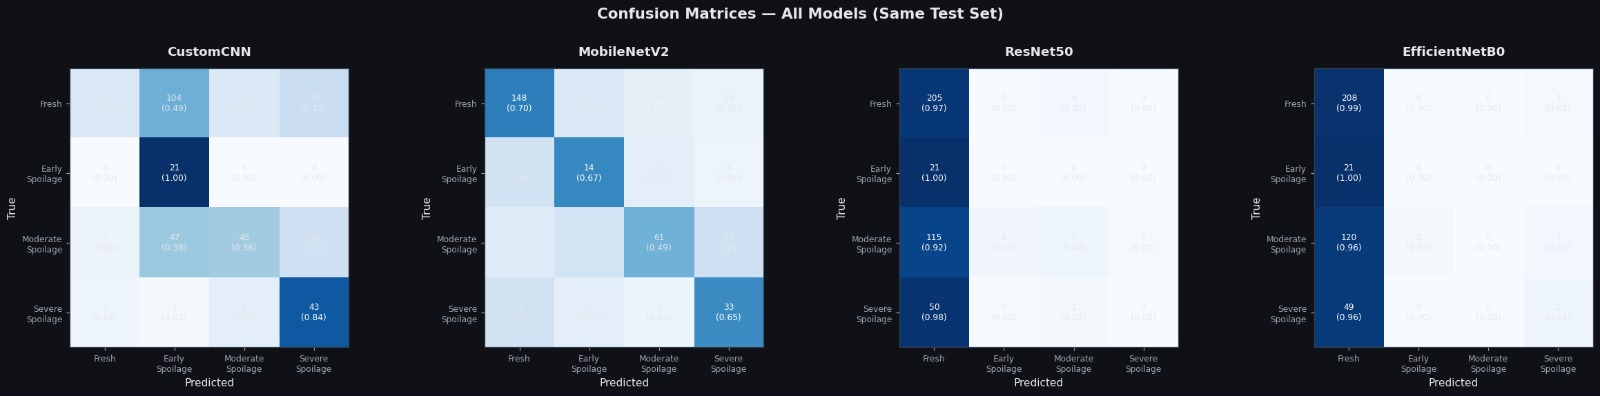
\includegraphics[width=1\textwidth]{Figures/confusion_matrices}
	\caption{Confusion Matrices for CustomCNN, MobileNetV2, ResNet50, and EfficientNetB0 on the same test set.}
	\label{fig:confusion_matrices_img}
\end{figure}

\begin{figure}[H]
	\centering
	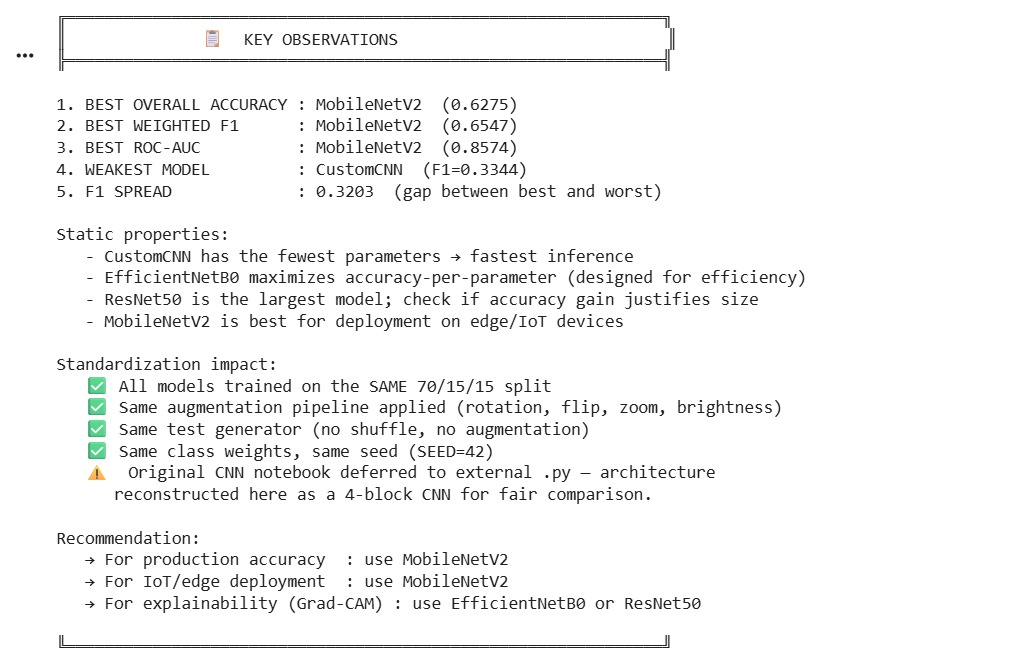
\includegraphics[width=0.8\textwidth]{Figures/key_observations}
	\caption{Key observations and summary of findings from the model evaluation.}
	\label{fig:key_observations_img}
\end{figure}

\begin{table}[H]
	\centering
	\caption{Key Observations from Comparative Analysis}
	\label{tab:key_observations}
	\begin{tabular}{|l|l|}
		\hline
		\textbf{Observation} & \textbf{Result} \\ \hline
		Best Overall Accuracy & MobileNetV2 (62.75\%) \\ \hline
		Best Weighted F1-Score & MobileNetV2 (65.47\%) \\ \hline
		Best ROC-AUC & MobileNetV2 (85.74\%) \\ \hline
		Fastest Lightweight Model & MobileNetV2 \\ \hline
		Weakest Overall Model & CustomCNN \\ \hline
		Largest Model Size & ResNet50 \\ \hline
	\end{tabular}
\end{table}

\section[ROC Curve and Per-Class Performance Analysis]{\textbf{ROC Curve and Per-Class Performance Analysis}}
ROC curve analysis was performed using a one-vs-rest classification strategy for all spoilage stages. The ROC curves indicate that MobileNetV2 achieved the highest Area Under Curve (AUC) values across most spoilage classes, demonstrating stronger class separability and prediction reliability. The model achieved particularly high ROC performance for Fresh and Severe Spoilage stages.

The CustomCNN model demonstrated acceptable ROC performance despite lower overall classification accuracy, indicating that the model was capable of learning important visual features but lacked strong class-wise generalization. ResNet50 and EfficientNetB0 produced weaker ROC curves for Early and Moderate Spoilage stages, suggesting difficulty in learning subtle spoilage transitions from the available dataset.

Per-class F1-score analysis revealed that Fresh samples were generally classified more accurately across all architectures because of their strong visual distinction. However, intermediate spoilage stages such as Early Spoilage and Moderate Spoilage were more difficult to classify due to overlapping visual characteristics and gradual spoilage progression. This highlights the complexity of multi-label food spoilage classification compared to conventional binary classification systems.

\begin{figure}[H]
	\centering
	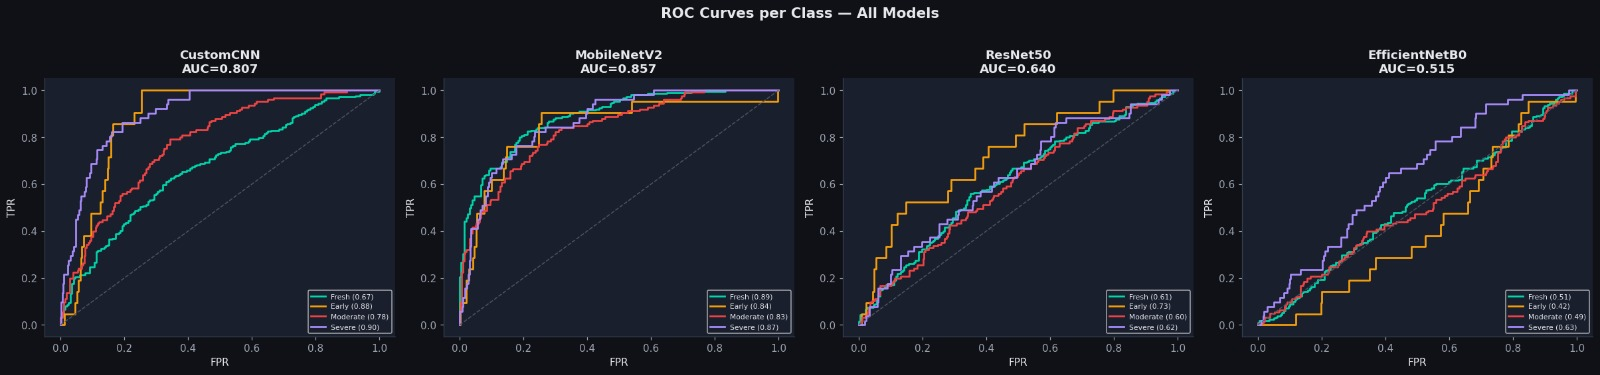
\includegraphics[width=1\textwidth]{Figures/roc_curves}
	\caption{ROC Curves per class for all evaluated deep learning models.}
	\label{fig:roc_curves_img}
\end{figure}


%Chapter 7
\chapter{CONCLUSION AND FUTURE SCOPE}
The proposed AI-based multi-label food spoilage detection system demonstrates the application of Deep Learning, Computer Vision, and Explainable AI techniques for automated food quality monitoring. The system was developed to classify fruits and vegetables into four spoilage stages: Fresh, Early Spoilage, Moderate Spoilage, and Severe Spoilage using image-based analysis. Multiple deep learning architectures including CustomCNN, MobileNetV2, ResNet50, and EfficientNetB0 were trained and evaluated using the same dataset and pre-processing pipeline for comparative analysis.

The experimental results indicate that MobileNetV2 achieved the best overall performance among all evaluated models with improved accuracy, F1-score, and ROC-AUC values. The lightweight architecture and efficient feature extraction capability of MobileNetV2 enabled better classification performance and faster inference compared to deeper architectures such as ResNet50 and EfficientNetB0. The confusion matrix and ROC analysis demonstrated that the proposed system was capable of performing effective multi-label spoilage classification, although intermediate spoilage stages remained more challenging because of overlapping visual characteristics.

The integration of Explainable AI using Grad-CAM improved model transparency and interpretability by highlighting image regions influencing predictions. The generated heatmaps demonstrated that the models focused on meaningful spoilage indicators such as discoloration, mold formation, bruises, and texture degradation during classification. The Streamlit-based web application further demonstrated the practical applicability of the proposed system for real-time food quality monitoring and prediction.

Although the IoT integration component is currently under development, the proposed framework successfully establishes the foundation for combining image-based deep learning and environmental sensing for food spoilage monitoring. The project demonstrates the potential of AI-driven systems for reducing food waste, improving food safety, and enabling intelligent food quality assessment in practical applications such as smart kitchens, grocery stores, warehouses, and inventory management systems.

\section[Future Scope]{\textbf{Future Scope}}
The future scope of the project includes complete integration of IoT-based environmental sensing using MQ-135 gas sensors and DHT11/DHT22 temperature-humidity sensors for real-time spoilage monitoring. Sensor fusion techniques can further improve prediction reliability by combining environmental conditions with image-based analysis. Additional food categories such as dairy products, packaged foods, and meat products can also be included to expand the applicability of the system.

Future work may also involve the use of larger and more diverse datasets to improve model generalization capability and classification accuracy for intermediate spoilage stages. Advanced architectures such as Vision Transformers (ViTs), multimodal learning models, and ensemble methods can be explored for improved performance. Cloud deployment, mobile application integration, and edge-AI implementation using embedded devices can further enhance the real-world usability of the proposed system.

\section[Learning Outcomes of the Project]{\textbf{Learning Outcomes of the Project}}
The project provided practical understanding of Deep Learning, transfer learning, image pre-processing, data augmentation, Explainable AI, and web application deployment techniques. The implementation process improved knowledge related to CNN architectures, transfer learning models, Grad-CAM visualization, and performance evaluation methods such as confusion matrix and ROC analysis.

The project also provided exposure to AI-based food quality monitoring systems and the integration of computer vision techniques with IoT-based monitoring frameworks. Practical implementation using TensorFlow, Keras, OpenCV, Streamlit, and Google Colab enhanced technical understanding of real-world AI application development workflows.


%% Uncomment the following 2 commands to add Appendix chapters
\appendix
\chapter*{APPENDIX}
\addcontentsline{toc}{chapter}{APPENDIX}
\markboth{APPENDIX}{APPENDIX}
\setcounter{section}{0}
\renewcommand{\thesection}{A.\arabic{section}}

The appendix presents selected implementation details, sample code snippets, and supporting outputs used during the development of the proposed AI-based multi-label food spoilage detection system. The implementation was carried out using Python in the Google Colab environment with TensorFlow, Keras, OpenCV, NumPy, Matplotlib, and Streamlit libraries. The appendix provides an overview of important code sections used for dataset preprocessing, model development, prediction generation, Explainable AI visualization, and web application deployment.

The developed system utilized transfer learning architectures such as MobileNetV2 and ResNet50 for spoilage classification. Image preprocessing operations including resizing, normalization, and augmentation were implemented to improve model training and generalization capability. Grad-CAM visualization techniques were also integrated to improve interpretability of model predictions. The following code snippets represent important implementation modules used in the project.

\section[Importing Required Libraries]{\textbf{Importing Required Libraries}}
The following libraries were imported for image preprocessing, deep learning model development, visualization, and performance evaluation. TensorFlow and Keras were used for model training, while OpenCV and NumPy were used for image processing operations.

\begin{lstlisting}[language=Python, caption=Importing Python libraries]
import tensorflow as tf
from tensorflow import keras
from tensorflow.keras import layers
from tensorflow.keras.applications import MobileNetV2, ResNet50

import cv2
import numpy as np
import matplotlib.pyplot as plt
\end{lstlisting}

\section[Dataset Preprocessing and Augmentation]{\textbf{Dataset Preprocessing and Augmentation}}
Image preprocessing and augmentation techniques were applied to improve dataset quality and increase data diversity. Augmentation operations such as rotation, zooming, horizontal flipping, and brightness adjustment helped reduce overfitting and improve model generalization capability.

\begin{lstlisting}[language=Python, caption=Dataset preprocessing and augmentation pipeline]
train_datagen = ImageDataGenerator(
    rescale=1./255,
    rotation_range=30,
    zoom_range=0.2,
    horizontal_flip=True,
    brightness_range=[0.7,1.3]
)

train_generator = train_datagen.flow_from_directory(
    '/content/data/train',
    target_size=(224,224),
    batch_size=32,
    class_mode='categorical'
)
\end{lstlisting}

\section[MobileNetV2 Model Architecture]{\textbf{MobileNetV2 Model Architecture}}
Transfer learning was implemented using MobileNetV2 pretrained on the ImageNet dataset. The pretrained backbone was used for feature extraction, while additional dense and dropout layers were added for spoilage stage classification.

\begin{lstlisting}[language=Python, caption=MobileNetV2 model construction]
base_model = MobileNetV2(
    include_top=False,
    weights='imagenet',
    input_shape=(224,224,3)
)

base_model.trainable = False

model = keras.Sequential([
    base_model,
    layers.GlobalAveragePooling2D(),
    layers.Dense(256, activation='relu'),
    layers.Dropout(0.4),
    layers.Dense(4, activation='softmax')
])
\end{lstlisting}

\section[Model Compilation and Training]{\textbf{Model Compilation and Training}}
The model was compiled using the Adam optimizer and categorical cross-entropy loss function. Training and validation datasets were used to evaluate model learning performance during multiple training epochs.

\begin{lstlisting}[language=Python, caption=Model compilation and training process]
model.compile(
    optimizer='adam',
    loss='categorical_crossentropy',
    metrics=['accuracy']
)

history = model.fit(
    train_generator,
    validation_data=val_generator,
    epochs=20
)
\end{lstlisting}

\section[Prediction Function]{\textbf{Prediction Function}}
The prediction pipeline processed uploaded food images and generated spoilage stage predictions using the trained deep learning model. The predicted class was obtained using the highest probability score from the softmax output layer.

\begin{lstlisting}[language=Python, caption=Prediction function for multi-label classification]
def predict_image(image_path):
    img = cv2.imread(image_path)
    img = cv2.resize(img, (224,224))
    img = img / 255.0
    img = np.expand_dims(img, axis=0)

    prediction = model.predict(img)
    predicted_class = np.argmax(prediction)

    return predicted_class
\end{lstlisting}

\section[Grad-CAM Visualization]{\textbf{Grad-CAM Visualization}}
Grad-CAM was implemented to generate heatmaps highlighting important image regions influencing the prediction process. The Explainable AI component improved transparency and interpretability of the deep learning model.

\begin{lstlisting}[language=Python, caption=Grad-CAM heatmap implementation]
def gradcam_heatmap(img_array, model):
    grad_model = tf.keras.models.Model(
        [model.inputs],
        [model.get_layer().output, model.output]
    )
\end{lstlisting}

\section[Streamlit Web Interface]{\textbf{Streamlit Web Interface}}
A Streamlit-based web application was developed to provide a simple and interactive interface for real-time spoilage prediction. Users could upload fruit or vegetable images and obtain spoilage predictions instantly.

\begin{lstlisting}[language=Python, caption=Streamlit web application snippet]
import streamlit as st

st.title("AI-Based Food Spoilage Detection")

uploaded_file = st.file_uploader(
    "Upload Fruit or Vegetable Image"
)

if uploaded_file is not None:
    st.image(uploaded_file)
\end{lstlisting}

\section[Performance Evaluation Metrics]{\textbf{Performance Evaluation Metrics}}
Different performance evaluation metrics such as Accuracy, Precision, Recall, and F1-Score were used to analyze the classification performance of the proposed models.

\begin{lstlisting}[language=Python, caption=Evaluation metrics import]
from sklearn.metrics import (
    accuracy_score,
    precision_score,
    recall_score,
    f1_score
)
\end{lstlisting}

\section[IoT Firmware: ESP8266 Blynk Integration]{\textbf{IoT Firmware: ESP8266 Blynk Integration}}
The IoT subsystem firmware was implemented on an ESP8266 microcontroller to interface with MQ-135 gas sensors and DHT11/DHT22 temperature-humidity sensors. The firmware integrates with Blynk cloud platform for real-time data transmission, local LCD display monitoring, and automated alert triggering. The following code represents the complete Arduino sketch for the IoT sensor integration module.

\begin{lstlisting}[language=C, caption=ESP8266 Blynk firmware for food spoilage monitoring]
#define BLYNK_TEMPLATE_ID "TMPL3K_iKoy77"
#define BLYNK_TEMPLATE_NAME "Food Spoilege detections"
#define BLYNK_AUTH_TOKEN "YrmWQOMAA8Fs9_0OmlkreAO5kcXZ3Vx3"

#include <Wire.h>
#include <LiquidCrystal_I2C.h>
#include <ESP8266WiFi.h>
#include <BlynkSimpleEsp8266.h>
#include <DHT.h>

// Mobile Hotspot Credentials
const char* ssid = "OnePlus Nord CE5 7DCA";
const char* password = "123456789";

// Pin Configurations
const int MQ3_PIN = A0;
#define DHTPIN D3
#define DHTTYPE DHT11
#define BUZZER_PIN D5
#define GREEN_LED D6
#define RED_LED D7

// Component Initializations
LiquidCrystal_I2C lcd(0x27, 16, 2);
DHT dht(DHTPIN, DHTTYPE);
BlynkTimer timer;

// Control Flags
bool alertTriggered = false;
bool displayToggle = true;

void monitorSystem() {
  // Read Sensor Telemetry
  int sensorValue = analogRead(MQ3_PIN);
  float humidity = dht.readHumidity();
  float temperature = dht.readTemperature();

  // Handle Sensor Errors Gracefully
  if (isnan(humidity) || isnan(temperature)) {
    humidity = 0;
    temperature = 0;
  }

  // Push Stream Data to Blynk Virtual Pins
  Blynk.virtualWrite(V2, sensorValue);    // Gauge / Chart Widget
  Blynk.virtualWrite(V3, temperature);    // Temp Value Widget
  Blynk.virtualWrite(V4, humidity);       // Humidity Value Widget

  String stageText = "FRESH";

  // 4-Stage State Machine Integration
  if (sensorValue > 750) {
    stageText = "SEVERE";
    digitalWrite(BUZZER_PIN, HIGH);
    digitalWrite(GREEN_LED, LOW);
    digitalWrite(RED_LED, HIGH);

    // Fire cloud automation event (Triggers Push and Email)
    if (!alertTriggered) {
      Blynk.logEvent("spoilage_alert");
      alertTriggered = true;
    }
  }
  else if (sensorValue > 500) {
    stageText = "MODERATE";
    digitalWrite(BUZZER_PIN, HIGH);
    digitalWrite(GREEN_LED, LOW);
    digitalWrite(RED_LED, HIGH);
    alertTriggered = false;
  }
  else if (sensorValue > 300) {
    stageText = "EARLY";
    digitalWrite(BUZZER_PIN, LOW);
    digitalWrite(GREEN_LED, HIGH);
    digitalWrite(RED_LED, LOW);
    alertTriggered = false;
  }
  else {
    stageText = "FRESH";
    digitalWrite(BUZZER_PIN, LOW);
    digitalWrite(GREEN_LED, HIGH);
    digitalWrite(RED_LED, LOW);
    alertTriggered = false;
  }

  // Local Output Interface Logic (Display toggles every 2 seconds)
  lcd.clear();
  if (displayToggle) {
    lcd.setCursor(0, 0);
    lcd.print("Gas Value: ");
    lcd.print(sensorValue);
    lcd.setCursor(0, 1);
    lcd.print("Stage: ");
    lcd.print(stageText);
  } else {
    lcd.setCursor(0, 0);
    lcd.print("Temp: ");
    lcd.print(temperature, 1);
    lcd.print(" C");
    lcd.setCursor(0, 1);
    lcd.print("Humid: ");
    lcd.print(humidity, 1);
    lcd.print(" %");
  }

  displayToggle = !displayToggle;
}

void setup() {
  Wire.begin(D2, D1);

  // Initialize Hardware Pin Registers
  pinMode(BUZZER_PIN, OUTPUT);
  pinMode(GREEN_LED, OUTPUT);
  pinMode(RED_LED, OUTPUT);

  // Enforce safe startup power values
  digitalWrite(BUZZER_PIN, LOW);
  digitalWrite(GREEN_LED, LOW);
  digitalWrite(RED_LED, LOW);

  lcd.init();
  lcd.backlight();
  lcd.clear();

  lcd.setCursor(0, 0);
  lcd.print("System Booting...");
  lcd.setCursor(0, 1);
  lcd.print("Waking Sensors...");

  dht.begin();

  // Initialize network socket parameters
  Blynk.begin(BLYNK_AUTH_TOKEN, ssid, password);
  timer.setInterval(2000L, monitorSystem);

  lcd.clear();
  lcd.setCursor(0, 0);
  lcd.print("System Online!");
  lcd.setCursor(0, 1);
  lcd.print("HARISH");
  delay(1500);
}

void loop() {
  Blynk.run();
  timer.run();
}
\end{lstlisting}

\textbf{Key Implementation Features:}
\begin{itemize}
    \item \textbf{Blynk Integration}: Cloud connectivity with template ID and auth token for remote monitoring and alert triggering.
    \item \textbf{Sensor Fusion}: Real-time acquisition of MQ-135 gas concentration (analog pin A0) and DHT11 temperature-humidity data (pin D3).
    \item \textbf{4-Stage Classification}: Threshold-based spoilage stage determination:
    \begin{itemize}
        \item \textbf{Fresh}: Gas $\leq 300$ ppm
        \item \textbf{Early Spoilage}: $300 < $ Gas $\leq 500$ ppm
        \item \textbf{Moderate Spoilage}: $500 < $ Gas $\leq 750$ ppm
        \item \textbf{Severe Spoilage}: Gas $> 750$ ppm
    \end{itemize}
    \item \textbf{Visual Feedback}: Tri-color LED indicator (Green=Fresh/Early, Red=Moderate/Severe) and piezo buzzer alarm for severe conditions.
    \item \textbf{LCD Display}: 16x2 I2C LCD alternates between gas/stage and temperature/humidity readings every 2 seconds.
    \item \textbf{Asynchronous Monitoring}: BlynkTimer executes sensor monitoring at 2-second intervals without blocking the main loop.
    \item \textbf{Alert Mechanism}: Spoilage alerts are logged to Blynk cloud platform triggering push notifications and email alerts when severe spoilage is detected.
\end{itemize}

The appendix demonstrates important implementation modules used during the development of the proposed food spoilage detection system. These implementation details support the methodologies and experimental results discussed in the previous chapters.%Appendix Chapter 1

\backmatter
\ifDrf
\else
\clearpage
\addcontentsline{toc}{chapter}{Bibliography}
\nocite{*}
\printbibliography%
\fi
\end{spacing}
\end{document}
